% =============================================================================
% paper.tex -- Who Gets Caught: Disclosure Rules, Liquidity and the Undetected Blockholder
%
% Compile (from the repo root, in this order):
%   xelatex -interaction=nonstopmode paper.tex
%   biber paper
%   xelatex -interaction=nonstopmode appendix.tex
%   xelatex -interaction=nonstopmode paper.tex
%   xelatex -interaction=nonstopmode paper.tex
%   xelatex -interaction=nonstopmode appendix.tex
% =============================================================================

\documentclass[11pt]{article}

\usepackage[margin=1in]{geometry}
\usepackage{amsmath,amssymb,amsthm}
\usepackage{setspace}
\usepackage{enumitem}
\usepackage{booktabs}
\usepackage{graphicx}
\usepackage{float}
\usepackage{xr}
\externaldocument[app:]{appendix}
\usepackage[hidelinks]{hyperref}
\usepackage[backend=biber,style=authoryear,natbib=true,maxcitenames=2,maxbibnames=99]{biblatex}
\addbibresource{paper.bib}
\setlength\bibitemsep{2.5pt}
\renewcommand*{\bibfont}{\small}

\setstretch{1.1}

\newtheorem{theorem}{Theorem}
\newtheorem{proposition}{Proposition}
\newtheorem{lemma}{Lemma}
\newtheorem{corollary}{Corollary}
\newtheorem{condition}{Condition}

\newcommand{\Eop}{\mathbb{E}}
\newcommand{\Prb}{\mathbb{P}}
\newcommand{\ind}{\mathbf{1}}
\newcommand{\Dact}{\Delta^{\mathrm{act}}}
\newcommand{\Sfl}{\mathsf{S}_F}
\newcommand{\Wrev}{\mathcal{W}}
\newcommand{\Grev}{\mathcal{G}}

\title{\textbf{Who Gets Caught: Disclosure Rules, Liquidity and the Undetected Blockholder}\\[0.3em]}
\author{Austin Li\\[0.25em]}
\date{This draft: 3 September 2026}

\begin{document}
\pagestyle{myheadings}
\markboth{Who Gets Caught}{Liquidity and the Undetected Blockholder}
\maketitle

%==============================================================================
\begin{abstract}
\noindent At fixed trading policies the engagement premium equals the premium wedge times the
probability that a bidder enters against an engaged blockholder. At the median five-round
calibration node and $\kappa=0.5$, bidder entry on silent pooled histories is several times as high
as entry on tape-detected pooled histories. The entry identity and the ordering at a fixed
fundamental posterior mean are PROVED; the calibrated multiple is NUMERICAL. The filing and the
trading tape detect opposite blockholders: the rule catches the fast builders who place the fewest orders,
while the tape is more likely to detect the slow builders who place many. On the calibration,
cutting the clock from ten rounds to five lowers the engagement premium by under one percent in
thin markets and by 17.5 to 54.3 percent in liquid ones, a NUMERICAL result. At fixed policies and
liquidity, tightening either dial is a Blackwell improvement of the market's experiment, a PROVED
result. At the paper's order size the tape is an exact erasure channel, and more liquidity is a
garbling of that channel, also PROVED. At $\kappa=0.5$, the re-pricing of histories that remain pooled is 93.2 to
98.0 percent of a shorter clock's net cut leg at every non-null clock node, a NUMERICAL result. The
empirical measurement is descriptive, with the post-minus-pre differences labelled
ESTIMATED. Among initial Schedule 13D campaigns with readable stakes from 2021 to 2025, the median
stake at filing is $13.1$ percent of class before the February 2024 clock change and $12.8$ percent
after. The share filed within five business days rises from $32.7$ to $75.9$ percent.
\end{abstract}

\newpage

%==============================================================================
\section{Introduction}
\label{sec:intro}
%==============================================================================

A blockholder who learns that a company is worth more than the market price can sell, wait, or try
to change the company. If she builds a large enough position while she waits, the law makes her
disclose it. In the United States, Section 13(d) requires a Schedule 13D from a beneficial owner of
more than 5 percent of a registered equity class who does not qualify for or elect Schedule 13G.
Until February 2024 the initial filing period was ten calendar days; it is now five business days
\citep{SEC2023}. The stake threshold and the filing clock split histories into a flagged cell, where
the filing has landed, and a pooled cell, where the market reads order flow. The filing and the tape
are two detection technologies. The rule catches fast builders with weakly fewer building rounds,
while the tape is more likely to identify slow builders with more building rounds
(Lemmas~\ref{app:lem:detection} and~\ref{app:lem:upper-set}).

The first result is an entry identity. If the price and bidder entry are measurable functions of
public information, then the engagement premium equals the premium wedge times the probability that
the bidder enters against a blockholder who is in fact engaged. Equivalently,
$\Dact=\Delta_m\Prb(\mathsf B=1,a=1)=\Delta_m\omega_V e_V$, where $\omega_V$ is the Voice mass and
$e_V$ is bidder entry conditional on Voice. The same identity holds within each public cell, and
$\omega_V$ is free of liquidity and the disclosure rule at fixed policies
(Lemma~\ref{app:lem:entry-identity}). On a silent pooled history, bidder entry is weakly higher than
on a tape-detected pooled history with the same fundamental posterior mean, and strictly higher when
the silent history's engagement posterior is below one (Lemma~\ref{app:lem:entry-undetected}). At the
median five-round node and $\kappa=0.5$, entry on silent pooled histories is 16.9 times entry on
tape-detected pooled histories (NUMERICAL).

At the fixed policies used in the calibration, liquidity raises the engagement premium. At the
paper's order size, one more unit of liquidity erases more building marks. A Voice type with $n$
building rounds has probability
$(\kappa/2)^n$ of remaining silent in the pooled cell (Lemma~\ref{app:lem:detection}). The exact
liquidity representation writes the derivative of the pooled premium as minus one half of the
premium wedge times the total marginal value of one more revealed round
(Lemma~\ref{app:lem:g3}). The one-crossing lemma applied to the record's coefficients shows that the
pooled premium is strictly increasing above a root below $0.15$ at every calibration node
(Lemma~\ref{app:lem:one-crossing}, NUMERICAL). At the median five-round node, the engagement premium
at $\kappa=0.85$ is 1.23 times its level at $\kappa=0.15$. Cutting the clock from ten rounds to five
lowers the engagement premium by 0.58 percent at the thin endpoint and by 45.4 percent at the liquid
endpoint at that node; at the liquid endpoint the effect runs from 17.5 to 54.3 percent across the
threshold ladder.

Tightening either disclosure dial weakly improves the market's control-date experiment in
Blackwell's order at a fixed liquidity (Theorem~\ref{app:thm:blackwell}). The flagged-tuple decoder
is required to recover each newly flagged type and reproduce the looser experiment. The strictness
criterion is PROVED (Corollary~\ref{app:cor:blackwell-strict}). On the calibration, the five-round
positive-mass threshold cuts are strict, the null ten-round threshold cuts are
Blackwell-equivalent, and the clock comparison is non-null (NUMERICAL). A Blackwell order at fixed
liquidity does not sign the liquidity sensitivity of the engagement premium. It orders level
experiments at one $\kappa$, while a rule change also changes the weight and composition of the
pooled cell.

The two dials change that sensitivity through the pooled share and the pool's composition. The
factorisation $\mathcal S=(1-\Omega)\mathcal S_P$ separates the pooled share from the pool's own
sensitivity (Proposition~\ref{app:prop:factorisation}). For either dial, the tighter rule lowers total
sensitivity exactly when its weight and composition ratios have product at most one
(Theorem~\ref{app:thm:clock} and Corollary~\ref{app:cor:caught-threshold}). The composition ratio is
governed by the net cut leg, which includes both the newly flagged histories and the re-pricing of
the histories that remain pooled (Corollaries~\ref{app:cor:caught}
and~\ref{app:cor:caught-threshold}). At $\kappa=0.5$, re-pricing accounts for 93.2 to 98.0 percent of
the net cut leg across the five non-null clock nodes.

The calibration uses order size two, $H=10$, the five threshold nodes, and $\kappa$ from $0.15$ to
$0.85$ in steps of $0.01$. The three-round clock is a grid extension. It flags exactly the same
histories as the five-round clock at every threshold node. The ten-round nodes are one pool and
serve as boundary checks. The benchmark one-step deviation bound is NUMERICAL at all fifteen nodes.

The registered empirical analysis gives institutional magnitudes for the stake and clock. It does
not measure market inference directly. The population is initial Schedule 13D campaigns from 2021
to 2025, taking one subject firm and trigger date as the campaign, without screening by Item 4 text,
and reading the maximum percentage across reporting persons. Stakes are readable for $91.6$ percent
of campaigns. The post-minus-pre differences in the stake at filing $B^F$ are labelled ESTIMATED.
The share filed within five business days rises from $32.7$ percent before the February 2024 clock
change to $75.9$ percent after, and the median trigger-to-filing delay falls from $7.0$ to $5.0$
business days. The comparison has no control group and identifies no causal effect.

The contribution is to join three literatures that usually hold different pieces fixed. Trading
models in the Kyle tradition study what order flow reveals \citep{Kyle1985,GlostenMilgrom1985}.
Work on blockholder liquidity studies exit, voice, and monitoring \citep{Maug1998,KahnWinton1998}.
Disclosure models study thresholds or fixed filing horizons \citep{BackEtAl2018,CorumLevit2019}.
Here the threshold and clock jointly choose which informed histories leave the pool, while the tape
separately identifies building marks. This makes entry against an engaged blockholder, inference
from silence, and the liquidity effect of the rule part of one accounting system.
Section~\ref{sec:lit} gives the institutional setting and related literature.
Section~\ref{sec:model} states the model. Section~\ref{sec:results} states each result with its
label. Section~\ref{sec:calibration} gives the numerical results. Section~\ref{sec:empirics}
presents the descriptive evidence, and Section~\ref{sec:conclusion} closes. The proofs and full
hypothesis lists are in the appendix.

%==============================================================================
\section{Institutional setting and related literature}
\label{sec:lit}
%==============================================================================

\subsection{The disclosure rule and its two margins}
\label{sec:institutional}

Section 13(d) requires beneficial owners of more than five percent of a registered equity class
to report their holdings. Investors with an activist intent or who do not qualify to report on
Schedule 13G must file Schedule 13D, disclosing their stake and purpose. The statutory initial
filing window was ten calendar days until the SEC amendments effective February 5, 2024 shortened
it to five business days \citep{SEC2023}. The threshold determines which holdings trigger a filing.
The clock determines how long a crossed position can remain in the pooled cell. Other disclosure
systems also vary these two margins, so the distinction is not tied to one statutory change.

The theoretical model abstracts this institution into two margins, defining the window margin
$T$ in discrete trading rounds. The clock starts when the stake reaches $\tau$, and the filing
lands $T$ trading rounds later. The numerical comparison between $T=10$ and $T=5$ below is a
comparative static across trading-round windows in the model, rather than a calibrated replica
of the calendar-day to business-day reform. Filing early is outside the model. The pooled cell
describes information available to the market makers who set prices. Other parties may learn
about accumulation through separate channels before a filing, as \citet{Zeng2026} documents
for target managers and stock-surveillance vendors. That possibility does not change the public
filing partition studied here.

\subsection{Exit, voice, and liquidity}
\label{sec:lit-exit-voice}

The classic trade-off originates with \citet{Hirschman1970}. \citet{Coffee1991} and
\citet{Bhide1993} argue that liquidity weakens governance by letting blockholders sell instead of
fight; \citet{Maug1998} reverses the logic. Liquid markets let a monitor recoup the costs of
engagement through informed trading, and with an endogenous stake liquidity raises monitoring.
\citet{KahnWinton1998} show the sign of the trading motive depends on whether engagement deepens the
blockholder's information advantage; \citet{FaureGrimaudGromb2004} make price informativeness and
insider incentives complements; \citet{AdmatiPfleiderer2009} make exit itself a disciplining threat.
On the empirical side, \citet{EdmansFangZur2013} find more liquid targets shift from voice to exit,
and \citet{NorliOstergaardSchindele2015} find liquidity predicts the incidence of costly voice.

This literature uses different meanings of liquidity, so its comparative statics do not map to
one common question. It also focuses on monitoring and trading rather than the disclosure
partition faced by a bidder. The formal object analysed here is the liquidity sensitivity of
the engagement-related component of the expected takeover premium, $\Dact = \Delta_m \Eop[\pi p]$,
when the legal rule sorts histories into flagged and pooled cells. It omits the baseline entry
term $m_0 \Eop[p]$, which can move with liquidity when entry moves. The factorisation and
comparative statics apply specifically to this engagement component rather than to total
takeover premia or shareholder welfare.

\subsection{Trading, disclosure, and the market for control}
\label{sec:lit-microstructure}

The trading model uses discrete order flow from the Kyle tradition \citep{Kyle1985,
GlostenMilgrom1985}, following the formulation in \citet{EdmansGoldsteinJiang2015}. It also uses the
feedback between prices and real decisions \citep{EdmansGoldsteinJiang2012, BondEdmansGoldstein2012,
Goldstein2023}. \citet{GrossmanHart1980} make the takeover premium the welfare object for dispersed
minority shareholders, and \citet{BurkartGrombPanunzi1998} show why higher premia protect them.

Several theory papers study related information splits. In \citet{KyleVila1991}, pooling comes
from the trader's mixing rather than a legal rule. \citet{CollinDufresneFos2015} and
\citet{CollinDufresneFos2016} study informed blockholder trading when the trader's presence is
known. \citet{BackEtAl2018} has a fixed disclosure horizon in a continuous-time Kyle model, where
a shorter horizon changes the scale of noise-trading volatility. The legal threshold and clock
here instead change which histories the market pools before a bidder acts.

\citet{CetemenCisternasKolbViswanathan2026} studies how blockholders time trades and coordinate
through market signals. \citet{Corum2025} limits how much of a stake can be traded before
disclosure but does not separate the threshold from the clock. \citet{CorumLevit2019} and
\citet{OrdonezCalafiBernhardt2022} study disclosure thresholds without a distinct window margin.
\citet{BurkartLee2022} studies the takeover premium while leaving anonymous pre-disclosure
toehold accumulation outside its model.

\subsection{Structural and empirical work on activism}
\label{sec:lit-structural}

Structural work estimates campaign costs, reputation, disclosure form, and takeover outcomes.
\citet{Gantchev2013} estimates the sequential costs of campaigns. \citet{JohnsonSwem2021} models
reputation when buying and filing occur together. \citet{AlbuquerqueFosSchroth2022} studies the
13D-versus-13G choice with announcement returns. \citet{CelentanoLevine2025} models activism,
takeovers, and managerial discipline with a fixed disclosure threshold. These models do not
separate a threshold margin from a filing clock. Empirical work links engagement campaigns to
acquisitions and returns \citep{BravJiangPartnoyThomas2008,GreenwoodSchor2009,
BechtFranksGrantWagner2017}. \citet{Zeng2026} measures information that target managers receive
before the public filing.

Recent work studies the clock change directly. \citet{PolkBuchheitRileyStone2024} uses pre-rule
variation in filing delays, while \citet{Trivedi2026} compares filings around the new rule. The
empirical measurement reports the stake at filing and realised filing delays before and after the
statutory change. The theory studies the threshold and clock as separate fixed-policy changes to
market inference.

%==============================================================================
\section{The model}
\label{sec:model}
%==============================================================================

\subsection{The object and the partition}
\label{sec:object}

The disclosure rule divides the market's information into two cases. A stake threshold $\tau$
and a window margin $T$ determine whether the filing has arrived by the control decision. In
the \emph{flagged} cell, the market sees the stake and the intention to engage. In the
\emph{pooled} cell, it sees only order flow and must infer whether an informed blockholder is
trading. The cells are exhaustive. The outcome of interest is the expected engagement-related
premium $\Dact(\kappa,\tau,T)$, its two cell averages $M_F$ and $M_P$, and their liquidity
sensitivities. A lower threshold is a tighter threshold margin; a shorter window is a tighter
window margin.

The model uses the discrete order-flow structure of \citet{Kyle1985} and
\citet{EdmansGoldsteinJiang2015}, competitive prices as in \citet{GlostenMilgrom1985}, and the
takeover premium as the dispersed shareholder's control-outcome measure in the spirit of
\citet{GrossmanHart1980}. The model adds the legal partition to these elements.

\subsection{Timing}
\label{sec:timing}

Trading dates are $d=0,\ldots,H$. Nature draws the standalone value and the blockholder's
signal. A cutoff vector then maps the signal into one of three plans. Exit sells the initial
stake on date zero and holds nothing thereafter. Hold keeps the initial stake. Voice builds
toward a signal-dependent target and carries the engagement indicator $a=1$. Only Voice can
cross the disclosure threshold.

On each date, a binary order mark records whether the Voice path schedules a building purchase. The
strategic order attached to that mark and the independent noise order form observed flow. Market
makers set the date's pooled price from the flow history and the fact that no filing has yet landed.
The blockholder pays the pooled price for the scheduled change in the stake. The path does not
respond to realised flow or prices.

For a Voice path, the clock starts at the first date $c$ on which the stake reaches $\tau$, and the
filing date is $f=c+T$ in trading rounds when $f\leq H$. The within-date order is explicit. The
blockholder pays the corresponding pooled price for every scheduled purchase through date $f$,
including the purchase that determines $B^F=B(s,f)$. The filing then lands. The blockholder pays the
flagged price for the remaining purchase $Q^F=b^*(s)-B^F$. The bidder acts after this update. If no
filing lands by $H$, the bidder acts on the pooled control-node history.

\subsection{Primitives}
\label{sec:primitives}

The firm's standalone value is $v\sim N(\mu_v,\sigma_v^2)$. The blockholder observes
$s=v+\varepsilon$, where $\varepsilon\sim N(0,\sigma_\varepsilon^2)$ is independent of $v$.
Thus $s\sim N(\mu_v,\sigma_s^2)$, with
$\sigma_s^2=\sigma_v^2+\sigma_\varepsilon^2$, and
\[
\Eop[v\mid s]=\mu_v+\beta(s-\mu_v),
\qquad
\beta=\frac{\sigma_v^2}{\sigma_v^2+\sigma_\varepsilon^2}.
\]
The analytic model uses the full signal line. The computations retain
$s\in[\mu_v-6\sigma_s,\mu_v+6\sigma_s]$ and renormalise the truncated Gaussian law on that
interval. A potential bidder has an independent shock $\xi\sim N(0,\sigma_\xi^2)$, mean synergy
$\bar S$, and entry cost $K>0$. Engagement adds $\Delta_V\geq0$ to standalone value and changes
the takeover premium from $m_0$ to $m_1$, where $\Delta_m=m_1-m_0>0$. The restriction
$m_0\geq0$ gives a unique continuous pricing root (Lemma~\ref{app:lem:pricing-root} in the appendix).

The Voice target follows the strictly increasing algebraic sigmoid used in the computations,
\[
b^*(s)=b_0+(\bar b-b_0)G\!\left(\frac{s-\mu_v}{\sigma_s}\right),
\qquad
G(x)=\frac{1+x/\sqrt{1+x^2}}{2}.
\]
Its accumulation length is
\[
n(s)=\operatorname{clip}\!\left(
\left\lceil n_{\rm scale}(H+1)
\left[1-G\!\left(\frac{s-\mu_v}{\sigma_s}\right)\right]\right\rceil,
1,H+1\right),
\]
which is weakly decreasing in $s$. The Voice stake path is
\[
B_V(s,d)=b_0+\bigl(b^*(s)-b_0\bigr)
\min\!\left\{1,\frac{d+1}{n(s)}\right\}.
\]
Exit has $B_E(s,-1)=b_0$ and $B_E(s,d)=0$ from date zero onward. Hold keeps $B_H=b_0$.
The threshold satisfies $b_0<\tau$. The first crossing is
$c_j(s;\tau)=\inf\{d:B_j(s,d)\geq\tau\}$, with value $+\infty$ if there is none, and
$D=\ind\{a=1,c+T\leq H\}$.

The order mark and order size are distinct. The mark
\[
g_{jd}(s)=\Gamma\bigl(B_j(s,d)-B_j(s,d-1)\bigr)\in\{0,1\},
\qquad
\Gamma(x)=\ind\{x\geq\bar\gamma\},
\]
is a building-purchase indicator. Its strategic order has size two noise lumps,
$q_{jd}(s)=2\bar z\,g_{jd}(s)$. Independent noise takes the values $-\bar z$, $0$, and
$+\bar z$, with probabilities $\kappa/2$, $1-\kappa$, and $\kappa/2$. Noise orders are
independent across dates and independent of the primitive draws. Observed pooled flow is
$X_d=q_{jd}+z_d$. Higher $\kappa$ is a noisier, more liquid market.

Under Exit, the blockholder sells the initial stake at the pooled date-zero price but leaves no
order mark. This is a model assumption. The public statistic records buy-side stake building, not
all signed inventory changes, and therefore keeps Exit and Hold in the same mark class. Modeling
signed liquidation would add a third strategic-order support and create a different information
experiment from the five-flow experiment studied here.

A pooled history records $(X_0,\ldots,X_d)$ and whether the filing has landed. A filing reports
$F=(B^F,a=1)$, and the flagged tuple adds the residual order, $\Sfl=(B^F,Q^F,a=1)$. Institutionally,
Item 4 of Schedule 13D requires disclosing the purpose of the acquisition and any plans or proposals
regarding future purchases. In the model, the public tuple $\Sfl$ captures this requirement: the filing
reveals the accumulated stake $B^F$, the activist's scheduled remaining purchase $Q^F = b^*(s) - B^F$
toward her target, and the engagement commitment $a=1$. This is a stronger information set than a
filing alone: Item 4 motivates the disclosure of plans, and the model takes the residual order and
the engagement commitment as exactly disclosed, which a filing does not guarantee. At the control
node, public information is the pooled history if $D=0$ and $\Sfl$ if $D=1$.
 The bidder's shock remains private. The engagement posterior is
$\pi(\mathcal I)=\Prb(a=1\mid\mathcal I)$ and equals one after a filing. The bidder enters with
probability
\begin{equation}
\label{eq:entry}
p(\mathcal I)=1-\Phi\!\left(
\frac{P+K+m_0+\pi\Delta_m-\bar S}{\sigma_\xi}
\right).
\end{equation}
With $\mathsf B$ the entry indicator, the terminal shareholder payoff is
\begin{equation}
\label{eq:Y}
Y=(1-\mathsf B)(v+a\Delta_V)+\mathsf B(P+m_0+a\Delta_m),
\end{equation}
and the competitive control-node price solves $P(\mathcal I)=\Eop[Y\mid\mathcal I]$. Earlier
pooled prices are tower expectations of the solved control-node payoff. Positive-probability
histories use Bayes' rule. The pricing map assigns a fixed full-support reference belief to an
empty mark-path history.

For plan $j$, the blockholder evaluates
\[
U_j(s)=\Eop\!\left[b_j^*(s)Y-C_j^{\rm trade}-a_jC_j(s)\mid s,j\right].
\]
The trading cost sums each position change times the price specified by the within-date timing.
The engagement cost is positive for Voice and zero for Exit and Hold. A weakly ordered cutoff
vector maps the signal into Exit, Hold, or Voice. The calibration uses the resulting cutoff
vector as its baseline policy and freezes it across the comparative statics. The blockholder
executes the selected path without responding to realised prices or flow. The single probability
space, finite menu, Borel policy objects, legal-clock rules, bounded pinned kernel, and fixed-policy
comparison are conditions (S1) to (S11) in the appendix. The independent ternary noise law stated
above is the common noise channel in (S12). The control-node convention in (S13) makes public
information exactly the flagged tuple on the flagged cell and the displayed pooled history on the
pooled cell, up to pinned prices. The flagged-tuple decoder in (S14) uses the strictly increasing
terminal target to recover the signal; the filing-tuple paragraph in Section~\ref{sec:primitives}
states the public content that supports this assumption. Conditions (S1) to (S14) apply whenever a
result cites the full standing-condition range.

\subsection{The order-size choice}
\label{sec:ordersize}

A stake-building order should be large enough to move outside an ordinary noise order, but not so
large that its sign reveals the blockholder in every round. Two noise lumps are a simple middle
scale. A building purchase is twice the size of one liquidity order, yet a noise sale can still
offset half of it and produce the same net flow as an idle blockholder facing a noise buy. The model
preserves one camouflage event while most flows reveal whether stake building occurred.

Flow takes the five values
$\{-\bar z,0,\bar z,2\bar z,3\bar z\}$. A building date produces
$\{\bar z,2\bar z,3\bar z\}$ and an idle date produces
$\{-\bar z,0,\bar z\}$. The supports meet only at $\bar z$. This single overlap makes higher
liquidity a garbling of lower liquidity and gives the pooled premium a polynomial form in
$\kappa$.

Proposition~\ref{app:prop:trichotomy} gives the full channel comparison (PROVED). With one noise
lump, $b=1$, higher liquidity is not a garbling of lower liquidity at interior nodes on any
nondegenerate mark-path set. With two noise lumps the channel is an exact, non-trivial erasure
family in liquidity. With three or more noise lumps every order mark is decoded, so all liquidity
nodes are Blackwell-equivalent. Two noise lumps are therefore the unique positive integral choice
that keeps camouflage while ordering liquidity by erasure. The normalisation is a transparency
choice: it isolates one ambiguous flow value without making every building mark public.

\subsection{Fixed policies and the two dials}
\label{sec:fixed-policies}

Every theoretical comparison holds the plan menu, cutoff vector, and execution paths fixed while
the disclosure rule $(\tau,T)$ moves. Each comparison holds $\kappa$ fixed across the two rules.
The numerics hold the solver's baseline policy fixed throughout. These comparisons isolate the market's
information problem rather than a policy response by the blockholder. The formal outcome is the
engagement-related component of the expected takeover premium,
\[
\Dact \;=\; \Delta_m\,\Eop\bigl[h(\mathcal I_H)\bigr], \qquad
h(\mathcal I) = \pi(\mathcal I)\,p(\mathcal I),
\]
omitting the baseline entry term $m_0\,\Eop[p]$. The cell averages are $M_F=\Delta_m\Eop[h\mid D=1]$
and $M_P=\Delta_m\Eop[h\mid D=0]$ with $D$ the disclosure indicator, the flagged weight is
$\Omega=\Prb(D=1)$, and the sensitivities are $\mathcal S=|\partial_\kappa\Dact|$ and
$\mathcal S_P=|\partial_\kappa M_P|$. The two dials act through the weight legs
\[
W_\tau \;=\; \frac{1-\Omega(\tau',T)}{1-\Omega(\tau,T)}
\quad(\tau' < \tau),
\qquad
W_T \;=\; \frac{1-\Omega(\tau,T')}{1-\Omega(\tau,T)}
\quad(T' < T),
\]
and the composition legs $C_\tau = \mathcal S_P(\tau',T)/\mathcal S_P(\tau,T)$ and
$C_T = \mathcal S_P(\tau,T')/\mathcal S_P(\tau,T)$, both unsigned.

By Lemma~\ref{app:lem:bf-monotone} in the appendix, under fixed policies, because Voice stakes are
weakly increasing in the calendar date and crossing dates are unchanged, shortening the window
margin lands the filing weakly earlier on every path flagged under both windows, and on those
paths the stake at filing $B^F$ weakly falls. The shorter window can also flag paths that the longer one leaves in the pool, so the set of
filers can change as well. The empirical section states this
pathwise monotonicity next to the measured stakes and draws nothing causal from the pairing.

%==============================================================================
\section{Results at fixed policies}
\label{sec:results}
%==============================================================================

Each statement reports its status as PROVED, NUMERICAL, or ESTIMATED. PROVED marks an analytic
result. NUMERICAL marks a result on the grid named at the point of claim. ESTIMATED marks a
descriptive estimate with its design and uncertainty. The appendix states the full hypothesis
lists cited below.

\subsection{The partition and the two-cell decomposition}
\label{sec:partition}

\noindent\textsc{Label: PROVED.}\par
\begin{lemma}[Disclosure partition; Appendix Section~\ref{app:sec:partition-factorisation}, Lemma~\ref{app:lem:partition}]
\label{lem:partition}
Under the standing conditions of Section~\ref{sec:model}, the disclosure indicator
$D = \ind\{a = 1,\ c(\tau) + T \le H\}$ is a measurable function of the control-node history,
and the flagged cell $\mathcal C_F = \{D = 1\}$ and the pooled cell $\mathcal C_P = \{D = 0\}$
are disjoint, cover the space, and are read off the observed history. No restriction on the
mass of either cell is used: $\Omega$ may be $0$ or $1$, and then the empty-weight cell is
null, possibly empty.
\end{lemma}

\noindent\textsc{Label: PROVED.}\par
\begin{lemma}[Two-cell decomposition; Appendix Section~\ref{app:sec:partition-factorisation}, Lemma~\ref{app:lem:two-cell}]
\label{lem:two-cell}
Under the same conditions, with the partition of Lemma~\ref{lem:partition} and whenever
$0 < \Omega < 1$,
\[
  \Dact \;=\; \Omega\,M_F \;+\; (1 - \Omega)\,M_P .
\]
At $\Omega = 1$ the identity reads $\Dact = M_F$ and at $\Omega = 0$ it reads $\Dact = M_P$;
in each of those cases the average over the null cell is undefined rather than zero, and it is
not determined by the law.
\end{lemma}

The partition is a measurable split of the history space. The decomposition integrates the bounded
premium kernel over its two public cells. These identities precede any comparison of liquidity or
of disclosure rules.

\subsection{The entry identity}
\label{sec:entry-identity}

\noindent\textsc{Label: PROVED.}\par
\begin{lemma}[Entry identity; Appendix Section~\ref{app:sec:detection}, Lemma~\ref{app:lem:entry-identity}]
\label{lem:entry-identity}
Let the price $P(\mathcal I_H)$ and bidder-entry probability $p(\mathcal I_H)$ be measurable
functions of the public information set, let $a$ be the type's engagement indicator, and let the
public disclosure cells belong to $\mathcal I_H$. Assume the finite-premium and fixed-policy
conditions (S9) to (S11). Write $\omega_V=\Prb(a=1)$ and, when $\omega_V>0$,
$e_V=\Eop[p(\mathcal I_H)\mid a=1]$. Then
\begin{equation}
\label{eq:entry-identity-main}
\Dact=\Delta_m\omega_Ve_V=\Delta_m\Prb(\mathsf B=1,a=1).
\end{equation}
For either positive-mass public cell $\mathcal C$ with positive Voice mass,
\begin{equation}
\label{eq:entry-identity-cell-main}
M_{\mathcal C}=\Delta_m\omega_{V\mid\mathcal C}e_{V\mid\mathcal C}.
\end{equation}
If the relevant Voice mass is zero, the premium is zero and the conditional entry probability is
undefined. At fixed policies, $\omega_V$ is independent of both $\kappa$ and the disclosure rule.
\end{lemma}

The identity follows from the tower property because $p(\mathcal I_H)$ is publicly measurable. It
turns the engagement premium into a probability of bidder entry against a blockholder who is in
fact engaged. Liquidity and the rule can move that probability, but not the Voice mass, when
policies are fixed.

\subsection{Information is monotone in the rule}
\label{sec:blackwell}

\noindent\textsc{Label: PROVED.}\par
\begin{theorem}[Tightening either disclosure dial; Appendix Section~\ref{app:sec:blackwell}, Theorem~\ref{app:thm:blackwell}]
\label{thm:blackwell}
Fix a common $\kappa\in[0,1]$ and fixed policies, and assume conditions (S1) to (S14). Compare either
$b_0<\tau'<\tau$ at a common clock or $T'<T$ at a common threshold. At the control date, tag each
output by its public cell and show the flagged tuple on the flagged branch and the pooled history on
the pooled branch. The tighter experiment is weakly more informative in Blackwell's order about the
type and about $(v,a)$. A type-independent Markov kernel reproduces the looser output from the
tighter output, up to prior-null outputs. The flagged-tuple decoder in (S14) is required because it
recovers the type on the tighter rule's flagged region. No positive-mass condition on either cell
is needed.
\end{theorem}

\noindent\textsc{Label: PROVED.}\par
\begin{corollary}[Posterior engagement risk; Appendix Corollary~\ref{app:cor:blackwell-posterior}]
Under (S1) to (S14) and the comparison in Theorem~\ref{thm:blackwell}, the tighter rule weakly lowers
expected posterior variance of engagement. The same holds for any square-integrable function of the
type.
\end{corollary}

\noindent\textsc{Label: PROVED.}\par
\begin{corollary}[The two-parameter Blackwell chain; Appendix Corollary~\ref{app:cor:blackwell-chain}]
If the active order is two noise lumps and $0<\kappa_L<\kappa_H<1$, the tighter rule at
$\kappa_L$ Blackwell-dominates either rule at $\kappa_H$. This combines the rule comparison with the
pooled garbling in Lemma~\ref{lem:garbling}.
\end{corollary}

\noindent\textsc{Label: PROVED.}\par
\begin{corollary}[Strictness criterion; Appendix Corollary~\ref{app:cor:blackwell-strict}]
Positive newly flagged mass, a nonatomic signal on that cut, and a finite looser pooled range make
the Blackwell order about the type strict.
\end{corollary}

\noindent\textsc{Label: NUMERICAL.}\par
On the calibration's five-round threshold ladder, every positive-mass cut is strict. The ten-round
threshold cuts are null and their experiments are Blackwell-equivalent. The clock comparison is a
separate non-null comparison under Theorem~\ref{thm:blackwell}.

A Blackwell order at fixed liquidity does not sign the liquidity sensitivity of the engagement
premium. It compares level experiments at one $\kappa$, while the rule also changes the composition
and weight of the pooled cell whose derivative defines that sensitivity.

\noindent\textsc{Label: PROVED.}\par
\begin{lemma}[The flagged cell does not move with liquidity; Appendix Section~\ref{app:sec:partition-factorisation}, Lemma~\ref{app:lem:flagged-kappa-free}]
\label{lem:flagged}
Fix the cutoff policy and the execution policy, and let the disclosure rule be fixed. Under
the standing conditions, with the composed terminal target strictly increasing on the flagged
signal region almost surely, uniqueness of the inner pricing fixed point, $\Omega > 0$, and a
bidder entry rule whose probability given the public information set neither depends on $v$
beyond it nor moves the entry shock, the flagged tuple $\Sfl$ makes the pre-filing pooled
history conditionally independent of the primitive triple $(v,s,\xi)$, and the flagged
posterior, the flagged price, the entry probability and $M_F$ do not depend on $\kappa$. In
addition $\Omega$ does not depend on $\kappa$ at fixed policies.
\end{lemma}

The flagged tuple recovers the signal and pins the flagged posterior. The pre-filing pooled price
can still move with $\kappa$; the lemma concerns the flagged endpoint and weight.

\subsection{The tape}
\label{sec:garbling}

\noindent\textsc{Label: PROVED.}\par
\begin{lemma}[Erasure and garbling on the tape; Appendix Section~\ref{app:sec:pf-garbling}, Lemmas~\ref{app:lem:g1} and~\ref{app:lem:g2}]
\label{lem:garbling}
Fix a policy with $\Omega(\tau,T)<1$ and $\kappa\in(0,1)$ at order size two. Write $R$ for
the set of rounds whose flow differs from one lump $\bar z$.
\begin{enumerate}[label=(\alph*),leftmargin=2.4em,itemsep=2pt]
\item The value $\bar z$ carries likelihood ratio one across types, so $R$ is independent of
  the blockholder's type, and on $R$ the flow determines the blockholder's order mark. The
  pooled posterior after any pooled history is therefore the pooled type law conditioned on
  the marks the history reveals, and nothing else.
\item For $0 < \kappa < \kappa' < 1$ there is a Markov kernel, not depending on the type, that
  carries the law of every pooled history at $\kappa$ into its law at $\kappa'$: the pooled
  experiment at $\kappa'$ is a garbling of the pooled experiment at $\kappa$, in the sense of
  \citet{Blackwell1953}.
\end{enumerate}
\end{lemma}

The appendix constructs the kernel by deleting revealed rounds and redrawing the surviving
coordinates. The pooled expectation of a convex or concave kernel is monotone in $\kappa$ in the
direction set by its curvature. This argument needs no normality assumption. \citet{BackEtAl2018}
obtains a related ordering from a Gaussian mean-preserving spread of the market maker's posterior
mean, while \citet{Ganuzapenalva2010} uses dispersion orderings of signal structures.

\noindent\textsc{Label: PROVED.}\par
\begin{lemma}[Detection; Appendix Section~\ref{app:sec:detection}, Lemma~\ref{app:lem:detection}]
\label{lem:detection}
Fix a date $d$ and a positive-probability pooled history. Assume that only Voice plans carry
positive order marks, each Voice building round carries mark one and strategic order
$2\bar z$, the common noise channel (S12) holds, and the pooled history and its pinned posterior are
public under (S6), (S8), and (S13). Flows $2\bar z$ and $3\bar z$ reveal a building mark, so the
engagement posterior is one on every pooled history containing either value. Flows $-\bar z$ and
zero reveal a zero mark, while $+\bar z$ is the only ambiguous value. For a Voice type with
$N_d$ building rounds through date $d$,
\begin{equation}
\label{eq:detection-silence-main}
\Prb(\text{no building mark revealed through }d\mid\theta)
=\left(\frac{\kappa}{2}\right)^{N_d}.
\end{equation}
If that type remains pooled, this event is a silent history.
\end{lemma}

One revealed building mark identifies engagement on a pooled history. On a pooled history without
such a mark, Voice remains observationally pooled with Exit and Hold. For a fixed Voice type, the
probability of no revealed mark weakly rises with liquidity.

\subsection{Who gets caught}
\label{sec:detection-caught}

\noindent\textsc{Label: PROVED.}\par
\begin{lemma}[Upper set; Appendix Section~\ref{app:sec:detection}, Lemma~\ref{app:lem:upper-set}]
\label{lem:upper-set}
Suppose the Voice target is weakly increasing in the signal, its accumulation length is weakly
decreasing, Voice occupies an upper interval of signals, and its stake and mark paths have the menu
form in Section~\ref{sec:primitives}. Under the timing and noise conditions (S4), (S5), (S7), and
(S12), the date-$d$ flagged signal set is an upper set. A higher Voice signal crosses weakly earlier
and has weakly fewer building rounds through any date. The probability that the tape reveals no
building mark is therefore weakly highest among the Voice types the rule flags, and is strictly
higher when the building-round counts differ and $\kappa>0$.
\end{lemma}

\noindent\textsc{Label: PROVED.}\par
\begin{lemma}[Silence; Appendix Section~\ref{app:sec:detection}, Lemma~\ref{app:lem:silence}]
\label{lem:silence}
Compare nested rules under a common prior, common fixed policies, and common liquidity. Assume the
tighter rule removes a positive-mass upper set of engaged types from the looser pool; the surviving
pooled types have the same type-conditional likelihood under both rules; $\Eop[v\mid s]$ is weakly
increasing and pooled flow is conditionally independent of $v$ given $s$; and the displayed pooled
history has positive probability under both rules. On every such common pooled history, including
every silent history with that positive probability, the tighter rule weakly lowers both the
engagement posterior and the posterior mean of the fundamental. The appendix gives the exact
strictness conditions.
\end{lemma}

\noindent\textsc{Label: PROVED.}\par
\begin{lemma}[Entry against the undetected]
\label{lem:entry-undetected}
Appendix Section~\ref{app:sec:detection}, Lemma~\ref{app:lem:entry-undetected}. Assume the unique
pinned pricing root. Assume the normal bidder-entry rule in equation~\eqref{eq:entry} and the
appendix's added engagement-price condition. The pricing root is
strictly increasing in both the fundamental posterior mean and the engagement posterior, while
bidder entry at that root is strictly decreasing in both. Holding the fundamental posterior mean
fixed, entry on a silent pooled history is therefore weakly higher than on a tape-detected pooled
history, and is strictly higher when the silent history's engagement posterior is below one.
\end{lemma}

The filing rule and the tape sort Voice types in opposite directions. The filing flags an upper set
with fewer building rounds. More building rounds give the tape more chances to reveal Voice. A
tighter rule also changes the inference drawn from the pooled histories that remain.

\subsection{The exact liquidity representation}
\label{sec:liquidity-representation}

\noindent\textsc{Label: PROVED.}\par
\begin{lemma}[Exact liquidity representation; Appendix Section~\ref{app:sec:pf-garbling}, Lemma~\ref{app:lem:g3}]
\label{lem:liquidity-representation}
For a positive-mass pooled cell at order size two, let $\Grev(S)$ be the expected premium kernel
after the order marks on rounds in $S$ are revealed. With $\varepsilon=\kappa/2$,
\begin{equation}
\label{eq:liquidity-representation-main}
M_P=\Delta_m\sum_S(1-\varepsilon)^{|S|}\varepsilon^{H+1-|S|}\Grev(S),
\end{equation}
where each $\Grev(S)$ is free of $\kappa$. The pooled premium is a polynomial and
\begin{equation}
\label{eq:liquidity-derivative-main}
\partial_\kappa M_P=-\frac{\Delta_m}{2}
\sum_{k=0}^{H}(1-\varepsilon)^k\varepsilon^{H-k}c_k.
\end{equation}
Each coefficient $c_k$ sums the changes $\Grev(S\cup\{d\})-\Grev(S)$ over one more revealed round.
Thus the derivative of the pooled premium in $\kappa$ is minus half the premium wedge times the
total marginal value of one more revealed round. Concavity of the reduced-form kernel makes the
derivative weakly positive; convexity reverses the sign.
\end{lemma}

\noindent\textsc{Label: NUMERICAL.}\par
\begin{corollary}[The engagement premium rises with liquidity on the calibration]
\label{cor:monotone-premium}
On the order-size-two, $H=10$ calibration with $T\in\{3,5,10\}$, the five threshold nodes and
$\kappa\in[0.15,0.85]$, the one-crossing lemma applied to the record's coefficients gives one root
below $0.15$ at every node. The pooled premium, and hence the engagement premium, is strictly
increasing in $\kappa$ throughout the stated grid. This application of
Lemma~\ref{app:lem:one-crossing} is NUMERICAL.
\end{corollary}

\subsection{The two dials}
\label{sec:dials}

\noindent\textsc{Label: PROVED.}\par
\begin{proposition}[Factorisation of liquidity sensitivity; Appendix Section~\ref{app:sec:partition-factorisation}, Proposition~\ref{app:prop:factorisation}]
\label{prop:factorisation}
Assume conditions (S1) to (S11), an interior partition at the policy under consideration, the
flagged-endpoint invariance in Lemma~\ref{lem:flagged}, and differentiability of
$\kappa\mapsto M_P$. Then
\begin{equation}
\label{eq:factorisation}
\mathcal S(\kappa,\tau,T)=\bigl(1-\Omega(\tau,T)\bigr)\mathcal S_P(\kappa,\tau,T)
\end{equation}
exactly. The same factor scales total variation over any liquidity grid without a differentiability
assumption. At order size two, Lemma~\ref{lem:liquidity-representation} makes $M_P$ a polynomial, so
the point derivative exists on the interior.
\end{proposition}

The disclosure rule first chooses the share that remains pooled. It then chooses the type
composition of that pool. The factorisation separates these weight and composition effects.

\begin{condition}[Composition at a threshold pair]
\label{cond:D}
Let $b_0<\tau'<\tau$ at a common clock. The pair satisfies Condition~\ref{cond:D} at $\kappa$ if
$|\Wrev_{\tau',T}(\kappa)|\leq|\Wrev_{\tau,T}(\kappa)|$, using the coefficient sum in
Lemma~\ref{lem:liquidity-representation}. This is equivalent to $C_\tau\leq1$ under the erasure
representation.
\end{condition}

\noindent\textsc{Labels: PROVED and NUMERICAL.} Factorisation, the weight leg, and the closed-form
implication below are PROVED. The composition conclusion $C_\tau\leq1$ and the dial inequality
are NUMERICAL on the order-size-two, $H=10$, $T=5$ grid at frozen benchmark policy, for all four
adjacent threshold pairs and $\kappa\in[0.15,0.85]$ in steps of $0.01$.\par
\begin{theorem}[The threshold dial at fixed policies; Appendix Section~\ref{app:sec:pf-garbling}, Theorem~\ref{app:thm:g-threshold}]
\label{thm:threshold}
Fix the plan and cutoff policies and a window $T$, and take $b_0 < \tau' < \tau$ with
$0 < \Omega(\tau,T)$, $\Omega(\tau',T) < 1$ and $\mathcal S_P(\tau,T) > 0$. Assume the two-cell
decomposition and the $\kappa$-invariance of the flagged average, each with its own
hypotheses. Then:
\begin{enumerate}[label=(\Alph*),leftmargin=2.4em,itemsep=2pt]
\item \emph{Factorisation.} $\mathcal S = (1-\Omega)\,\mathcal S_P$ exactly, at every
  $\kappa \in (0,1)$.
\item \emph{Weight leg.} $\mathcal C_F(\tau,T) \subseteq \mathcal C_F(\tau',T)$ and every newly
  flagged history is generated by a Voice plan, so $\Omega(\tau',T)\geq\Omega(\tau,T)$ and
  $W_\tau\in[0,1]$. Equality holds when the threshold change reclassifies no history (almost surely).
\item \emph{Composition leg and the dial.} Under Condition~\ref{cond:D} at the pair and at
  $\kappa$, $C_\tau \le 1$, and therefore
  \begin{equation}
  \label{eq:threshold-dial}
  \frac{\mathcal S(\tau',T)}{\mathcal S(\tau,T)} \;=\; W_\tau\,C_\tau \;\le\; 1 .
  \end{equation}
\end{enumerate}
\end{theorem}

\noindent\textsc{Label: PROVED.}\par
\begin{theorem}[The clock dial at fixed policies; Appendix Section~\ref{app:sec:partition-factorisation}, Theorem~\ref{app:thm:clock}]
\label{thm:clock}
Fix the liquidity $\kappa$, the threshold margin $\tau$, and the plan and cutoff policies.
Compare two window margins $T' < T$. Assume $b_0 < \tau$, that Voice stake paths are weakly
increasing in the calendar date, that only Voice plans cross, $0 < \Omega(\tau,T) < 1$,
$0 < \Omega(\tau,T') < 1$, $\mathcal S_P(\kappa,\tau,T) > 0$, and the hypotheses of
Proposition~\ref{prop:factorisation} at both clocks, the differentiability of
$\kappa \mapsto M_P$ each instance carries included. Then:
\begin{enumerate}[label=(\roman*),leftmargin=2.4em,itemsep=2pt]
\item the weight leg attenuates: $0 < W_T \le 1$;
\item the sensitivity ratio factors as $\mathcal S(\kappa,\tau,T')/\mathcal S(\kappa,\tau,T)
  = W_T\,C_T$;
\item the shorter clock lowers noise sensitivity exactly when the product of the two legs is
  at most one,
  \[
  \mathcal S(\kappa,\tau,T') \;\le\; \mathcal S(\kappa,\tau,T)
  \qquad\Longleftrightarrow\qquad
  W_T\,C_T \;\le\; 1 .
  \]
\end{enumerate}
\end{theorem}

The two dials enter with different force. The threshold weight leg is PROVED. Its composition leg is
NUMERICAL on the order-size-two, $H=10$, $T=5$ grid at frozen benchmark policy, for four adjacent
threshold pairs and $\kappa\in[0.15,0.85]$ in steps of $0.01$. The clock result is PROVED as an
exact equivalence. The model does not sign $C_T$, so the effect of a shorter clock depends on which
histories leave the pooled cell. Because $W_T>0$, the attenuation criterion is equivalent to
$C_T\leq1/W_T$, and the right-hand side is at least one.

\subsubsection*{The composition bands}
\label{sec:caught}

Fix the threshold margin $\tau$ and the policies, and compare $T' < T$ at a common $\kappa$.
Write $A = \mathcal C_P(\tau,T)$ for the pooled cell under the longer clock and
$B = \mathcal C_F(\tau,T')\setminus\mathcal C_F(\tau,T)$ for the histories the shorter clock
newly flags, with $\varphi = \Prb(B)/\Prb(A)$ the share of the pool that is caught. Write
$s_A = \partial_\kappa\Eop[h^{(T)} \mid A]$ for the pool's own noise sensitivity in kernel
units and $s_B$ for the \emph{net cut leg}: the derivative with respect to $\kappa$ of the
premium mass the shorter clock removes from the pool, per unit of caught mass, with the
survivors' re-pricing included. The caught-only leg $\widetilde s_B$ instead reads newly flagged
histories under the looser rule's kernel.

\noindent\textsc{Label: PROVED.}\par
\begin{corollary}[Who gets caught; Appendix Section~\ref{app:sec:caught}, Corollary~\ref{app:cor:caught}]
\label{cor:caught}
Under (C-1) to (C-3) of the appendix, with the clock theorem's hypotheses also applying, (C-1)
uses (S10) for liquidity entering only through the noise law and cites fixed policies separately as
(S11). Then:
\begin{enumerate}[label=(\roman*),leftmargin=2.4em,itemsep=2pt]
\item the cut is nested, $B \subseteq A$, $A\setminus B = \mathcal C_P(\tau,T')$, and the
  weight leg is $W_T = 1-\varphi$;
\item the cell masses do not depend on $\kappa$, so $\varphi$ does not either;
\item the cut identity holds exactly:
  \[
  s_A \;=\; (1-\varphi)\,s_{A\setminus B} + \varphi\,s_B,
  \]
  the longer clock's pooled sensitivity is the mass-weighted average of what the shorter clock
  leaves in the pool and what it takes out;
\item the composition ratio satisfies
  \[
  C_T\leq1
  \quad\Longleftrightarrow\quad
  (s_B-s_A)\bigl(\varphi s_B-(2-\varphi)s_A\bigr)\leq0.
  \]
  Thus $C_T\leq1$ exactly when $s_B$ lies weakly between $s_A$ and
  $((2-\varphi)/\varphi)s_A$. The attenuation criterion $W_TC_T\leq1$ holds exactly when
  $s_B$ lies weakly between $0$ and $(2/\varphi)s_A$;
\item under a common nonzero sign, $C_T\leq1$ is equivalent to
  $|s_A|\leq|s_B|\leq((2-\varphi)/\varphi)|s_A|$. The net cut leg must be at least as
  noise-sensitive as the pool and no more than that multiple.
\end{enumerate}
\end{corollary}

\noindent\textsc{Label: PROVED.}\par
\begin{corollary}[Who gets caught at the threshold margin; Appendix Section~\ref{app:sec:caught}, Corollary~\ref{app:cor:caught-threshold}]
\label{cor:caught-threshold}
At a common clock, replace the clock-indexed sets and kernels above by
$A_\tau=\mathcal C_P(\tau,T)$,
$B_\tau=\mathcal C_F(\tau',T)\setminus\mathcal C_F(\tau,T)$ and
$R_\tau=A_\tau\setminus B_\tau$, where $b_0<\tau'<\tau$. Under (C$\tau$-1) to (C$\tau$-3), the
cut is nested, its masses are free of $\kappa$, and the same accounting law holds:
\[
s_{A,\tau}=(1-\varphi_\tau)s_{R,\tau}+\varphi_\tau s_{B,\tau}.
\]
The composition condition $C_\tau\leq1$ holds exactly when the net cut leg lies weakly between
$s_{A,\tau}$ and $((2-\varphi_\tau)/\varphi_\tau)s_{A,\tau}$. Aggregate attenuation holds exactly
when it lies weakly between zero and $(2/\varphi_\tau)s_{A,\tau}$. Under (C$\tau$-4), which adds
(S12), (S13), order size two and interior liquidity, the composition condition is equivalent to
Condition~\ref{cond:D}.
\end{corollary}

\noindent\textsc{Label: PROVED.}\par
\begin{lemma}[The cut split at both margins; Appendix Section~\ref{app:sec:caught}, Lemma~\ref{app:lem:cut-split}]
\label{lem:cut-split}
For either non-null nested cut, let $h^-$ and $h^+$ be the looser and tighter kernels, let
$R=A\setminus B$, and orient the re-pricing term as
$\delta_{\rm cut}=\partial_\kappa\Eop[h^- -h^+\mid R]$. Under (S1) to (S11), the nesting and
differentiability hypotheses in the appendix give
\begin{equation}
\label{eq:cut-split-main}
s_B=\widetilde s_B+\frac{1-\varphi}{\varphi}\delta_{\rm cut}.
\end{equation}
The first term is the caught-only leg. The second is the re-pricing of histories that remain pooled
under both rules.
\end{lemma}

\noindent\textsc{Label: PROVED.}\par
\begin{lemma}[One crossing decides the composition band; Appendix Section~\ref{app:sec:caught}, Lemma~\ref{app:lem:one-crossing}]
\label{lem:one-crossing}
Under (S1) to (S13), take a non-null nested cut at order size two. Suppose each pool's coefficient
list changes sign once from negative to positive, their difference changes sign once from positive
to negative, and liquidity lies above the three positive roots of the reversed coefficient
polynomials. Then the two signed pooled slopes satisfy $0<s^+<s^-$ and
\[
s^-<s_B<\frac{s^-}{\varphi}<\frac{2-\varphi}{\varphi}s^-.
\]
The net cut leg lies strictly inside the composition band, so the tighter pool has strictly lower
liquidity sensitivity.
\end{lemma}

\noindent\textsc{Label: PROVED.}\par
\begin{lemma}[Distinct crossings reverse total sensitivity; Appendix Section~\ref{app:sec:caught}, Lemma~\ref{app:lem:reversal}]
\label{lem:reversal}
Under (S1) to (S13) and the factorisation hypotheses at both rules, suppose the two continuous
pooled slopes each cross zero once at distinct roots. There is then an open interval containing the
looser pool's root on which the tighter rule has strictly greater total liquidity sensitivity.
\end{lemma}

The two bands answer different questions. The composition band compares the two pooled
sensitivities. The wider aggregate band also credits the reduction in pooled mass. Both run on the
net cut leg, so survivors' re-pricing is part of the comparison rather than a residual left outside
it.

%==============================================================================
\section{The calibration}
\label{sec:calibration}
%==============================================================================

The calibration uses order size two and $H=10$. A seed policy at $\tau=0.05$, $T=5$, and
$\kappa=0.5$ supplies the Voice region. The threshold ladder uses the full-line signal quantiles
$0.1$, $0.3$, $0.5$, $0.7$, and $0.9$ of the stake-at-filing distribution under that seed policy.
The calculation clips signals only if a quantile crosses the computational support. The resulting
$\tau$ values run from $0.0924$ to $0.0970$. A second policy calculation at the median threshold,
$T=5$, $\kappa=0.5$, and $H=10$ gives the benchmark cutoff vector $k=(0.9425,1.8485)$. Expectation
calculations use the renormalised computational signal law stated in Section~\ref{sec:primitives}.
The clock grid is $T\in\{3,5,10\}$, and the liquidity grid has seventy-one nodes,
$\kappa=0.15$ to $0.85$ in steps of $0.01$. Every comparison in this section freezes the benchmark
plan menu, cutoff vector and stake paths.

\subsection{Premium levels and detection}

\noindent\textsc{Label: NUMERICAL.}\par
The engagement premium rises across the liquidity grid at every rule node. At the median threshold
and $T=5$, its value at $\kappa=0.85$ is 1.23 times its value at $\kappa=0.15$. This is the level
counterpart to Corollary~\ref{cor:monotone-premium}; the one-crossing lemma applied to the record's
coefficients places every relevant root below the grid.

Table~\ref{tab:detection-entry} separates bidder entry by public detection state at the median
five-round node. At $\kappa=0.5$, entry on silent pooled histories is 16.9 times entry on
tape-detected pooled histories. Silent pooled histories carry little mass, but their conditional
entry rate is high.

\begin{table}[H]
\centering
\caption{Bidder entry by detection state at the median threshold node and $T=5$ (NUMERICAL). Entry
is conditional on Voice within each state. The last column is the mass of pooled Voice histories
that are silent.}
\label{tab:detection-entry}
\small
\begin{tabular}{ccccc}
\toprule
$\kappa$ & Flagged & Pooled, tape-detected & Pooled, silent & Silent Voice mass \\
\midrule
0.15 & 1.2 percent & 3.4 percent & 58.8 percent & below 0.0001 percent \\
0.50 & 1.2 percent & 3.4 percent & 57.9 percent & 0.01 percent \\
0.85 & 1.2 percent & 3.4 percent & 57.3 percent & 0.11 percent \\
\bottomrule
\end{tabular}
\end{table}

\begin{figure}[H]
\centering
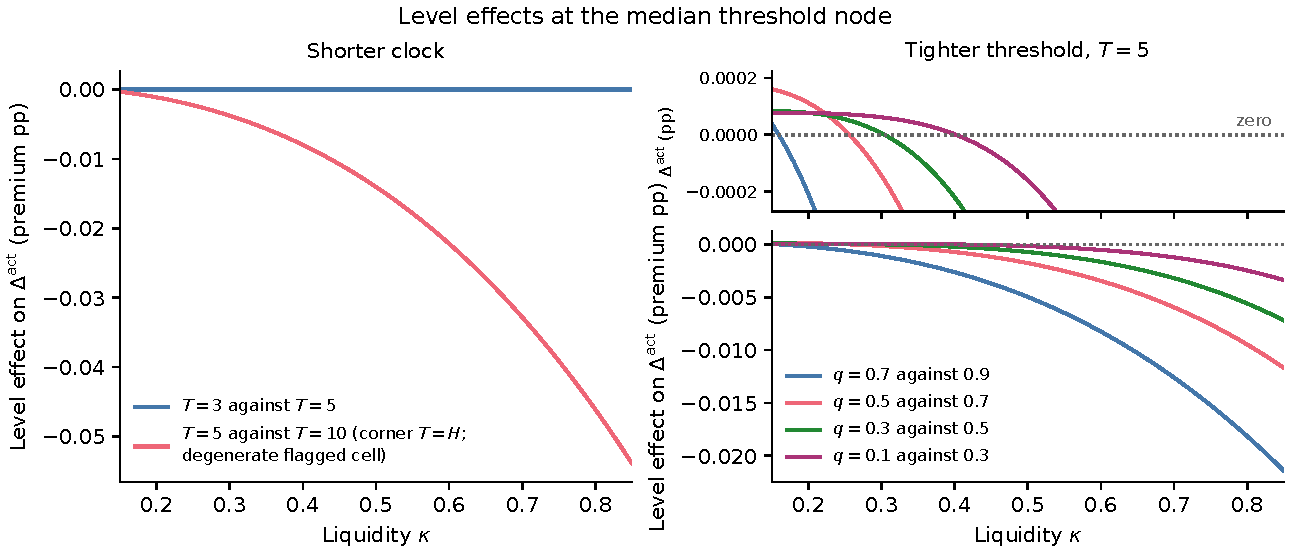
\includegraphics[width=0.96\textwidth]{figures/fig4_level_effects.pdf}
\caption{The level effect of the shorter clock and of the tighter threshold on the engagement
premium against liquidity $\kappa$ at the median node, with both clock pairs (NUMERICAL). The
three-round clock is a grid extension. The ten-round clock equals the horizon and is a one-pool
boundary.}
\label{fig:level-effects}
\end{figure}

At the median node, shortening the clock from $T=10$ to $T=5$ lowers the engagement premium by
0.58 percent at $\kappa=0.15$ and 45.4 percent at $\kappa=0.85$. At $\kappa=0.85$ the effect runs
from 17.5 to 54.3 percent across the five threshold nodes. The three-round and five-round clocks
flag exactly the same histories at every threshold node. For this grid extension, the median effect
is 0.00 percent at $\kappa=0.15$ and 0.00 percent at $\kappa=0.85$, and the cross-node range at
$\kappa=0.85$ is 0.00 to 0.00 percent.

For the four adjacent threshold cuts at $T=5$, the sign of the level effect is mixed over the
$\kappa$ region 0.15 to 0.40. Its largest magnitude below $\kappa=0.45$ is 5.99 percent. At the median
node and $\kappa=0.5$, the clock's negative level effect consists of a negative contribution from
newly caught histories and a larger negative re-pricing of survivors. The tighter threshold has a
negative contribution from newly caught histories that is partly offset by positive re-pricing of
survivors. These two level splits are NUMERICAL and sum to the corresponding engagement-premium
changes at every grid point.

\subsection{Liquidity sensitivity, the split and the bands}

\paragraph{The factorisation on the grid.} The largest pointwise residual
$|\mathcal S-(1-\Omega)\mathcal S_P|$ over the order-size-two, $H=10$ grid at frozen baseline
policies is $5.1\times10^{-17}$. The flagged weight is flat in $\kappa$ to exactly $0.0$ at every
node. Figure~\ref{fig:sensitivity} draws the median threshold quantile and reports both factors.

\begin{figure}[H]
\centering
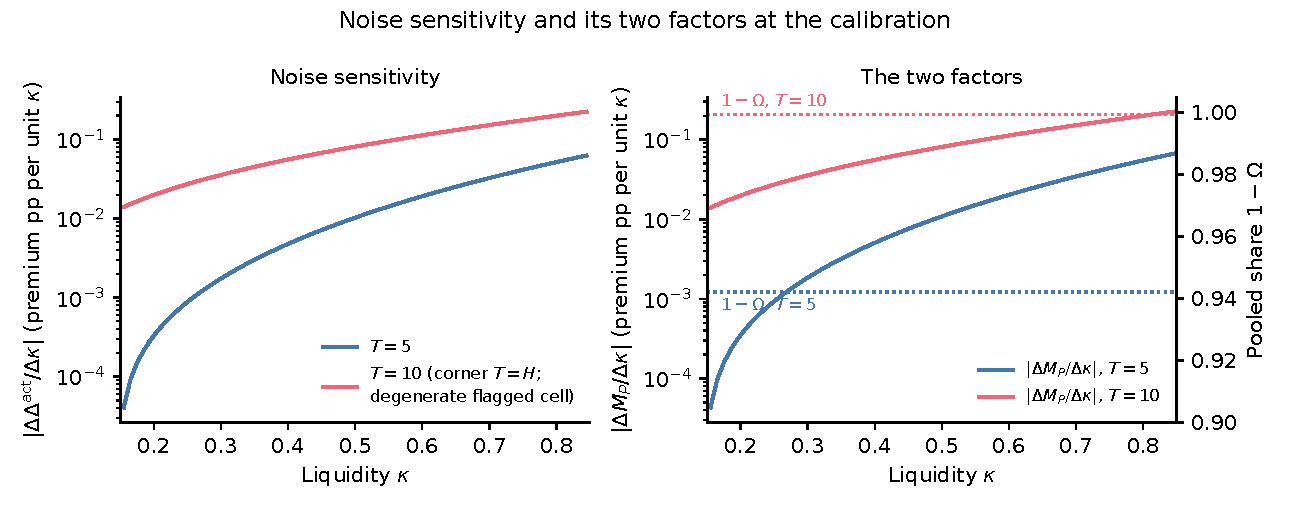
\includegraphics[width=0.95\textwidth]{figures/fig1_sensitivity_factors.pdf}
\caption{Noise sensitivity and its two factors against liquidity $\kappa$ at the calibration node
(the median threshold quantile, $\tau = 0.0945$), under both clocks, from the order-size-two
calibration record at frozen benchmark policy. Sensitivities are slopes over consecutive grid nodes
in premium percentage points per unit $\kappa$; the grid is $\kappa = 0.15$ to $0.85$ in steps of
$0.01$ with no gap. Left: $|\Delta \Dact / \Delta\kappa|$ (the finite-difference sensitivity).
Right: the two factors, the pooled finite-difference sensitivity $|\Delta M_P / \Delta\kappa|$ (left
axis, log scale) and the pooled share $1-\Omega$ (right axis, dotted), the factorisation $|\Delta
\Dact / \Delta\kappa| = (1-\Omega)|\Delta M_P / \Delta\kappa|$ holding to machine precision on every
node. At $H = 10$ the clock $T = 10$ is the corner $T = H$. Its flagged cell carries mass $\Omega =
6.8 \times 10^{-4}$ at every threshold node, below the code's degenerate-cell floor of $0.01$.}
\label{fig:sensitivity}
\end{figure}

\paragraph{The threshold dial on the grid.} The composition ratio is at most one at every adjacent
threshold pair in Table~\ref{tab:threshold}. This conclusion and the resulting dial inequality are
NUMERICAL on the order-size-two, $H=10$, $T=5$ grid at frozen benchmark policy, with
$\kappa\in[0.15,0.85]$ in steps of $0.01$. At $T=10$ every node is one pool, so the threshold cuts
are null boundary checks and both legs equal one. The weight leg at $T=5$ lies between $0.975$ and $0.977$, with reclassified mass $0.0232$
at each pair. The composition leg reaches $0.791$. The largest value of $W_\tau C_\tau$ is $0.772$,
for the change from the $0.5$-quantile threshold to the $0.3$-quantile threshold. The claim covers
only the named grid.

\begin{table}[H]
\centering
\caption{The threshold dial at fixed policies, from the revelation record (NUMERICAL, grid
$\kappa \in [0.15, 0.85]$ in steps of $0.01$, order size two, $H=10$, $T=5$, frozen
benchmark policy). Each row
tightens the threshold from the $\tau$ quantile in the second column to the tighter one in the
first. $W_\tau$ is the weight leg; $C_\tau$ runs over the whole $\kappa$ grid; the last column
is the largest product on the grid.}
\label{tab:threshold}
\begin{tabular}{cccccc}
\toprule
Tighter $\tau$ quantile & From & Window $T$ & $W_\tau$ & $C_\tau$ range & $\max_\kappa W_\tau C_\tau$ \\
\midrule
0.1 & 0.3 & 5 & 0.975 & $[0.279, 0.456]$ & 0.445 \\
0.3 & 0.5 & 5 & 0.975 & $[0.219, 0.791]$ & 0.772 \\
0.5 & 0.7 & 5 & 0.976 & $[0.029, 0.587]$ & 0.573 \\
0.7 & 0.9 & 5 & 0.977 & $[0.140, 0.633]$ & 0.618 \\
\bottomrule
\end{tabular}
\end{table}

\paragraph{The clock dial on the record.} The clock comparison is NUMERICAL on the order-size-two,
$H=10$ grid at frozen benchmark policy, with $\kappa\in[0.15,0.85]$ in steps of $0.01$, five
threshold nodes, and compares window margins $T=5$ against $T=10=H$ in discrete trading rounds.
This is a model comparison across trading-round horizons rather than a calibrated replica of the
statutory reform. The $T=10$ nodes are one-pool boundary checks, with flagged mass
$\Omega=6.8\times10^{-4}$ below the code's $0.01$ floor. Table~\ref{tab:window} shows that the shorter clock reduces total-variation
sensitivity to between $2$ and $69$ percent of its long-clock value. The composition ratio runs
from $0.024$ to $0.699$, while the weight leg reduces the pooled share by between $1.1$ and
$10.4$ percent.

\begin{table}[H]
\centering
\caption{The window record at fixed policies (NUMERICAL, $\kappa\in[0.15,0.85]$ in steps of
$0.01$, order size two, $H=10$, frozen benchmark policy): cutting the clock from $T = 10$ to $T = 5$ at
each threshold node. Sensitivities are total variations of $\Dact$ and $M_P$ over the $\kappa$
grid. At $H = 10$ the clock $T = 10$ equals the horizon and its flagged cell is degenerate
($\Omega = 6.8\times10^{-4}$, below the code's floor of $0.01$), so those nodes are one-pool
boundary checks.}
\label{tab:window}
\begin{tabular}{ccccc}
\toprule
$\tau$ quantile & $\Omega(\tau,5)$ & $W_T$ & $C_T$ & $W_T C_T$ \\
\midrule
0.1 & 0.10420 & 0.896 & 0.024 & 0.021 \\
0.3 & 0.08104 & 0.920 & 0.080 & 0.074 \\
0.5 & 0.05789 & 0.943 & 0.196 & 0.184 \\
0.7 & 0.03473 & 0.966 & 0.378 & 0.365 \\
0.9 & 0.01158 & 0.989 & 0.699 & 0.691 \\
\bottomrule
\end{tabular}
\end{table}

\paragraph{Who gets caught on the record.} On the five-node
clock-composition grid, the net cut leg lies strictly inside the corollary's
band and $C_T<1$ at every node (NUMERICAL, frozen benchmark policy, point derivatives at
$\kappa=0.5$, order size two, $H=10$, $T'=5$ against $T=10=H$, with the $T=10$ flagged cell
degenerate at every node because $\Omega=6.8\times10^{-4}<0.01$). The pool sensitivity is
$s_A=0.0040$ in kernel units, $s_B$ ranges from $0.039$ to $0.135$, the upper multiple ranges
from $18$ to $182$, and $C_T$ ranges from $0.013$ to $0.643$.

\begin{figure}[H]
\centering
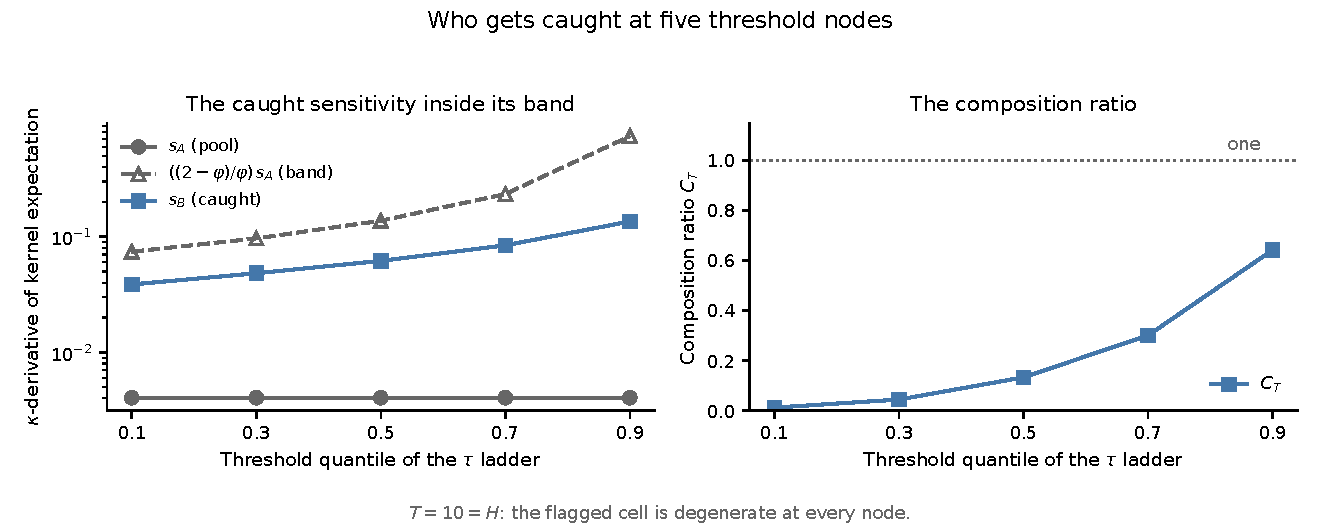
\includegraphics[width=0.95\textwidth]{figures/fig2_who_gets_caught.pdf}
\caption{The who-gets-caught record at five threshold nodes. The left panel places the net cut leg $s_B$
strictly between $s_A$ and $((2-\varphi)/\varphi)s_A$, and the right panel has $C_T<1$, at
every node (NUMERICAL, frozen benchmark policy, point derivatives at $\kappa=0.5$, order size
two, $H=10$, $T'=5$ against $T=10=H$, with the $T=10$ flagged cell degenerate at every node
because $\Omega=6.8\times10^{-4}<0.01$). The right panel marks $1$ as the ceiling.}
\label{fig:caught}
\end{figure}

\noindent\textsc{Label: NUMERICAL.}\par
The one-crossing lemma applied to the record's coefficients places the median clock cutoff at
$\kappa=0.146$ and the median five-round threshold cutoff at $\kappa=0.149$. Their printed
composition intervals therefore start at 0.15 and cover the full grid. Table~\ref{tab:cut-split}
reports the net cut split across every non-null node at $\kappa=0.5$.

\begin{table}[H]
\centering
\caption{The net cut split and composition intervals (NUMERICAL). Re-pricing share is the
survivors' re-pricing term divided by the net cut leg at $\kappa=0.5$ and is reported across every
non-null node of the stated margin.}
\label{tab:cut-split}
\small
\begin{tabular}{lccccc}
\toprule
Margin & Pairs & Max flagged mass & Re-pricing share & Cutoff & Starts \\
\midrule
Clock, $T=5$ against $T=10$ & 5 & 0.104 & 93.2 to 98.0 percent & 0.146 & 0.15 \\
Threshold, $T=5$ & 4 & 0.023 & 84.2 to 97.2 percent & 0.149 & 0.15 \\
\bottomrule
\end{tabular}
\end{table}

Inside a threshold pair's reversal interval the net cut leg crosses zero, so its re-pricing share
is undefined and is not reported there.

\noindent\textsc{Label: NUMERICAL.}\par
\paragraph{Remark.} At the median node the clock reversal interval is 0.02 to 0.02, where the
looser and tighter pooled sensitivities are \texttt{6.6e-09} and \texttt{2.0e-06}, compared with
\texttt{8.1e-04} and \texttt{1.1e-04} at $\kappa=0.5$; the median five-round threshold reversal
interval is 0.144 to 0.148.

\subsection{The benchmark policy and the numerical reconciliation}

\noindent\textsc{Label: NUMERICAL.}\par
At benchmark prices and beliefs, a one-step deviation changes only the plan at one signal on the
truncated support. Across the full design of 15 nodes and a mesh width of 1e-5, the largest bound is
\texttt{2.4e-04}; the largest bound among the five-round and ten-round nodes is also
\texttt{2.4e-04}. This is 0.63 percent of the payoff normaliser 0.038. The calculation implements
Proposition~\ref{app:prop:regret} under its stated deviation convention.

\begin{table}[H]
\centering
\caption{Benchmark one-step deviation bound (NUMERICAL). The benchmark pass, prices and beliefs are
fixed; the signal support is truncated; a cutoff takes the plan on its right.}
\label{tab:regret}
\begin{tabular}{cccccc}
\toprule
Design nodes & Mesh width & Largest bound & Largest, $T=5,10$ & Normaliser & Share \\
\midrule
15 & 1e-5 & \texttt{2.4e-04} & \texttt{2.4e-04} & 0.038 & 0.63 percent \\
\bottomrule
\end{tabular}
\end{table}

The reference belief on empty mark-path histories perturbs the coefficient calculations by at most
\texttt{2.7e-09}, below the smallest sign margin \texttt{1.1e-07}. The signs used by the exact
liquidity representation and the numerical record therefore agree.

%==============================================================================
\section{The empirics: the stake at filing and the clock}
\label{sec:empirics}
%==============================================================================

\subsection{Design and gates}
\label{sec:e1design}

The empirical layer is descriptive, reporting filing stakes and delays around the February 2024
rule change to provide institutional magnitudes for the model parameters rather than measuring
market inference directly. It identifies no effect, uses no control group, and makes no causal claim.
The design fixes the population and measurement before estimation. The measured object is the stake
at filing $B^F$, which the model produces at the filing date.

The population is every initial Schedule 13D filing (form types \texttt{SC 13D} and \texttt{SCHEDULE
13D}, both EDGAR spellings, no amendments) in the EDGAR quarterly form indexes from 2021 Q1 through
2025 Q4, with no screen on Item 4 purpose text. The unit is the campaign, one subject firm and
trigger date pair. The procedure collapses simultaneous group filings to the earliest acceptance.
The resulting sample has $4914$ campaigns. The procedure reads the stake from the cover page as the
percent of class and takes the maximum across reporting persons in a joint filing. The period split
is the rule date: pre if the trigger predates 2024-02-05, post otherwise. The delay of the clock
paragraph is the count of federal business days from the trigger date to the filing date.

The registered quality gates cover parsing, blind hand checks, and differential coverage. Readable
stakes cover $91.6$ percent of campaigns. The blind check reads sixty stratified campaigns and finds
zero material stake or trigger-date errors. The pre-to-post coverage gap is $7.0$ percentage points.
All three gates pass. The following subsection labels the post-minus-pre bootstrap differences
ESTIMATED; the registered design treats the remainder of the tables as descriptive statistics.

\subsection{The stake at filing}
\label{sec:e1results}

Table~\ref{tab:e1} reports $B^F$ by calendar year of the filing date and by period;
Figure~\ref{fig:e1} draws the distribution. Among campaigns with a readable stake, the median
is $13.1$ percent of class before the rule date and $12.8$ after, while the mean moves from
$22.3$ to $23.9$.

\noindent\textsc{Label: ESTIMATED.}\par
The post-minus-pre difference in the mean is $1.66$ percentage points with
a campaign-level percentile-bootstrap interval of $[0.20,3.11]$ based on $2{,}000$ draws and
seed 5. The median difference is $-0.30$ with interval $[-1.62,1.30]$.

\begin{table}[H]
\centering
\caption{The stake at filing $B^F$, percent of class, by calendar year of the filing date and
by period around the 2024-02-05 rule date. Campaigns with a readable stake; the coverage gate
E1-G1 passed at $91.6$ percent. The difference rows are post minus pre, campaign-level
bootstrap, $2{,}000$ draws, seed 5. Descriptive; no control group; no causal claim.}
\label{tab:e1}
\begin{tabular}{lccccc}
\toprule
 & $n$ & Mean & Median & P25 & P75 \\
\midrule
2021 & 1040 & 21.8 & 14.4 & 7.7 & 26.4 \\
2022 & 807 & 22.6 & 12.9 & 7.0 & 25.3 \\
2023 & 856 & 21.5 & 11.0 & 6.7 & 25.0 \\
2024 & 843 & 24.4 & 12.7 & 6.8 & 31.5 \\
2025 & 956 & 24.1 & 13.7 & 7.2 & 29.5 \\
\midrule
Pre (trigger before 2024-02-05)  & 2888 & 22.3 & 13.1 & 7.2 & 26.2 \\
Post (trigger from 2024-02-05)    & 1614 & 23.9 & 12.8 & 6.9 & 29.4 \\
\midrule
Difference in mean    & \multicolumn{5}{c}{$1.66 \; [0.20,\ 3.11]$} \\
Difference in median  & \multicolumn{5}{c}{$-0.30 \; [-1.62,\ 1.30]$} \\
\bottomrule
\end{tabular}
\end{table}

\begin{figure}[H]
\centering
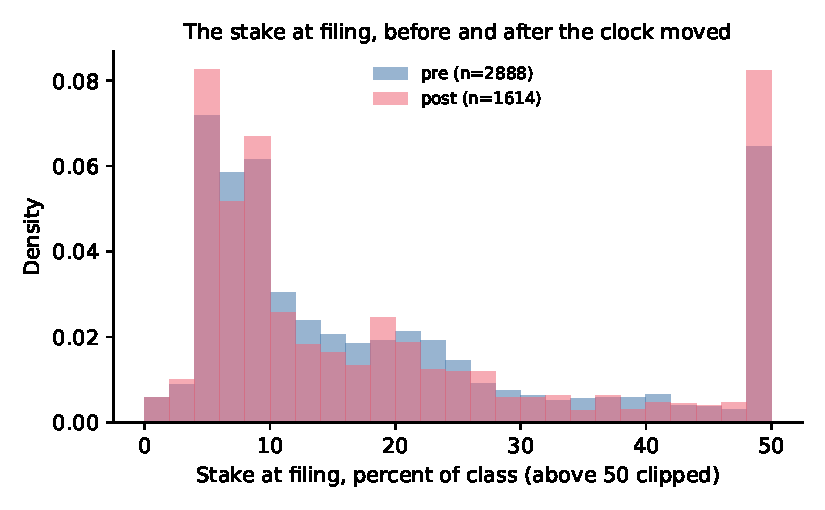
\includegraphics[width=0.62\textwidth]{figures/e1_stake.pdf}
\caption{The stake-at-filing distribution by period among campaigns with a readable stake,
from the campaign table behind Table~\ref{tab:e1}. The pre period has $n=2888$ and the post
period has $n=1614$. The medians are $13.1$ and $12.8$ percent of class. Descriptive; no
control group.}
\label{fig:e1}
\end{figure}

By Lemma~\ref{app:lem:bf-monotone} in the appendix, under fixed policies, a shorter window weakly
lowers the stake at filing on every path flagged under both windows. That statement is pathwise. The measured cross-section is not. The shorter clock can bring paths into the filing set that the
longer clock left in the pool, so the median and the mean of the filers can move either way. The
measured median difference is $-0.30$ percentage points, while the mean difference is $1.66$ points.
Table~\ref{tab:e1} reports their percentile-bootstrap intervals. This comparison is descriptive, and
the paper draws no causal conclusion from it. The rule date may coincide with other market changes,
so a before-and-after split carries no identification.

\subsection{The clock moved}
\label{sec:clock}

Table~\ref{tab:clock} documents the change in filing timing. It reports, by calendar year and by
period around the rule date, the share of campaigns filed within five
business days of the trigger and the median trigger-to-filing delay in federal business days.
Before the rule date, $32.7$ percent of campaigns were filed within five business days
(percentile-bootstrap interval $[31.1,34.3]$) and the median delay was $7.0$ business days;
after it, $75.9$ percent were filed within five business days ($[73.8,77.9]$) and the median
delay was $5.0$. By calendar year, the share within five business days rises from $27.8$
percent in 2021 to $39.0$ percent in 2023, then to $70.6$ percent in 2024 and $70.2$ percent in
2025. The median delay across those years is $7.0$, $7.0$, $6.0$, $5.0$, and $5.0$ days. The
statement is descriptive. It documents a change in realised timing at the rule date and
identifies no effect on another outcome.

The delay calculation uses all filings with a parsed trigger date and filing date. In the raw
records, two filings have a negative delay, reflecting typographical date errors
on the cover page, and $138$ filings have parsed trigger dates predating 2021 (the earliest reaching back
to 2010 with a delay of $2{,}870$ business days), reflecting multi-year legacy accumulations or late
disclosures. Retaining these filings preserves the registered descriptive protocol; because the primary
statistics are medians and shares within five business days, they are robust to extreme positive or
negative delays.

\begin{table}[H]
\centering
\caption{The filing clock, by calendar year of the filing date and by period around the
2024-02-05 rule date. The share is campaigns filed within five business days of the trigger;
the interval is a campaign-level bootstrap, $2{,}000$ draws, seed 5, reported for the two
period rows. Every campaign with a measured delay, no outcome screen. Descriptive.}
\label{tab:clock}
\begin{tabular}{lccc}
\toprule
 & Campaigns & Within 5 bus.\ days, \% & Median delay, bus.\ days \\
\midrule
2021 & 1167 & 27.8 & 7.0 \\
2022 & 903 & 33.9 & 7.0 \\
2023 & 962 & 39.0 & 6.0 \\
2024 & 918 & 70.6 & 5.0 \\
2025 & 964 & 70.2 & 5.0 \\
\midrule
Pre (before 2024-02-05)  & 3237 & 32.7 $[31.1,\ 34.3]$ & 7.0 \\
Post (from 2024-02-05)   & 1677 & 75.9 $[73.8,\ 77.9]$ & 5.0 \\
\bottomrule
\end{tabular}
\end{table}

%==============================================================================
\section{Conclusion}
\label{sec:conclusion}

A disclosure rule partitions histories before it changes market inference. At fixed trading
policies, the engagement premium is the premium wedge times the probability of bidder entry against
an engaged blockholder (Lemma~\ref{app:lem:entry-identity}, PROVED). Within pooled histories, entry
on a silent history is weakly higher than on a tape-detected history at a fixed fundamental
posterior mean. The filing and the tape detect opposite Voice types. The rule catches fast builders
with few orders, while the tape is more likely to identify slow builders with many orders
(Lemmas~\ref{app:lem:detection},
\ref{app:lem:upper-set}, and~\ref{app:lem:entry-undetected}, PROVED).

More liquidity erases more building marks. The pooled engagement premium is strictly increasing
above a root below the calibration grid at every node, and the shorter clock's effect on the
engagement premium grows sharply with liquidity (Lemma~\ref{app:lem:one-crossing}, NUMERICAL). At
the same time, tightening either policy dial weakly improves the market's control-date experiment
in Blackwell's order (Theorem~\ref{app:thm:blackwell}, PROVED). That order does not sign the
liquidity sensitivity of the premium.

The sensitivity results give the accounting behind the level result. Total liquidity sensitivity
is the pooled share times the pool's own sensitivity (Proposition~\ref{app:prop:factorisation},
PROVED). For either dial, the net cut leg determines whether the tighter rule lowers that
sensitivity. The net cut leg includes the histories newly caught by the rule and the re-pricing of
the histories left in the pool (Corollaries~\ref{app:cor:caught}
and~\ref{app:cor:caught-threshold}, PROVED). On the calibration, survivors' re-pricing supplies most
of that leg.

These comparisons hold the menu, cutoff vector and stake paths fixed. At benchmark prices and
beliefs, the largest one-step deviation bound across the fifteen design nodes is
\texttt{2.4e-04}, or 0.63 percent of the payoff normaliser (Proposition~\ref{app:prop:regret},
NUMERICAL). This is the quantitative check on the fixed benchmark policy under the stated
deviation convention.

The empirical measurement is descriptive, with the post-minus-pre differences labelled ESTIMATED.
Among initial Schedule 13D campaigns with readable stakes from 2021 to 2025, the median stake at
filing is $13.1$ percent of class before the 2024 clock change and $12.8$ percent after. Across all
measured delays, the share filed within five business days rises from $32.7$ to $75.9$ percent, while
the median delay falls from $7.0$ to $5.0$ business days. These measurements describe the stake at
filing and the change in realised filing timing at the rule date. They do not identify an effect of the
clock on the stake.

\printbibliography

\end{document}
